\documentclass[10pt]{article}
\usepackage{../../../local}
\usepackage{subcaption}
\usepackage{caption}
\usepackage{multirow}
\urlstyle{same}

\usepackage[style=numeric, sorting=none, maxnames=3]{biblatex}
\addbibresource{SHE.bib}

\newcommand{\classcode}{Physics 111B}
\newcommand{\classname}{SHE: Hall Effect in a Semiconductor}
\renewcommand{\maketitle}{%
\hrule height4pt
\large{Eric Du \hfill \classcode}
\newline
\large{SHE Report} \Large{\hfill \classname \hfill} \large{\today}
\hrule height4pt \vskip .7em
\small{Header styling inspired by CS 70: \url{https://www.eecs70.org/}}
\normalsize
}
\linespread{1.2}
\DeclareMathOperator*{\sgn}{sgn}
\begin{document}
	\maketitle
	\begin{abstract}
		In this lab, we investigate the Hall effect, and how it can be used to calculate fundamental
		constants such as the carrier mobilities and densities of a semiconductor. We use a hole-doped
		germanium crystal (which we will confirm to be so in the lab) as our semiconductor, and use the Van
		der Pauw technique to experimentally determine the resistivity. From these measurements, we determine
		the Hall coefficient, the hall mobility, the individual carrier mobitilies and densities and their
		relationship to temperature in this lab. We then discuss the nature and accuracy of our results to
		verify our experiment.        
	\end{abstract}
	\section{Introduction}
	This report concerns the SHE experiment in the Physics 111B Experimentation
	Laboratory. In this report, we will begin by detailing the theoretical background
	for the phenomena, then analyze the data we collect to verify our theoretical
	results. 
	\section{Theory}
	In this section, we will cover all the theory relevant to our experiment and our analysis. Unlike other
	labs, this lab is particularly theory heavy, so it is imperative that the underlying theory be understood
	so that the data and results may be effectively interpreted. As such, this lab report will follow a slightly
	different structure than the others: we will go over \textit{all} the requisite theory in this section,
	instead of saving some theory for the analysis. As it turns out, the analysis and results will be
	relatively straightforward,  
	\subsection{Conductors, Insulators and Semiconductors}
	Before discussing the hall effect, it is useful to outline the underlying physics of conductors,
	semiconductors and insulators, as the theoretical background will be important for our analysis performed
	later in the lab.\footnote{This is actually especially true for this lab, moreso than the other ones.} 
	To begin, the most important question to ask is: what actually causes current to flow through a material?
	Or, in other words, what causes a material to become electrically conductive? 
	
	Before tackling this question, we need to first examine the energy levels of electrons in a solid. In
	contrast to singular atoms, where the energy levels are discrete and separated by a known energy gap,
	the energy levels in a solid exist in \textit{energy bands}, separated by some energy gap \( E_g \). The
	reason this occurs is because unlike a singular atom, an electron not only feels electrostatic attraction
	to its host atom, but also to all the positively charged neighboring nuclei in the solid. 
	Thus, these extra electrostatic forces cause the electron to become "delocalized" in the material,  
	and thus the electrons now exist in an energy bands instead of levels. 

	To study current, we need to become intimately familiar with two particular energy bands, called the
	\textit{valence band} and the \textit{conduction band}. At absolute zero, due to the Pauli exclusion
	principle, electrons cannot occupy the same state, so electrons do the next best thing -- occupy all the
	lowest energy levels up to a certain energy, which we call the Fermi energy \( E_F \).
	All energy levels below this energy are occupied, and are what we define to be the \textit{valence band}. 
	The valence band is (mostly) filled at all times, at least for the temperature regimes we will be 
	working with. 

	By contrast, the conduction band is a band of allowed energy levels at which an electron is able to
	freely roam through the material. Because of this freedom, these electrons will move when a voltage
	difference is applied through the material, which manifests itself as measurable current. This energy
	band is generally unfilled, unlike the valence band. As such, this band exists at a higher energy than
	the valence band, and the difference between the highest energy in the valence band and the lowest energy
	in the conduction band is called the \textit{band gap}, denoted as \( E_g \). When an electron has energy
	greater than \( E_F + E_g \), then it has the ability to be promoted to the conduction band, and in
	doing so it also leaves behind a \textit{hole}, which can be thought of as a positron, or a positively
	charged electron. Because of this effect, holes and electrons in the conduction band come in pairs, a
	fact which will become useful later.   
	So, the study of current is effectively dictated by the transition of electrons between the valence and 
	conduction bands. Below, we study the structure of the valence and conduction bands inside a conductor, 
	an insulator, and finally a semiconductor.    

	First, we consider a conductor. By definition, conductors are materials that allow current to flow when
	even a small \( V > 0 \) is applied to both ends of the material.
	In order for this
	to happen, this would mean that there must exist electrons in the conduction band at all times; the
	only way for this to happen is if the valence and conduction band overlap, so that at any given
	temperature there are electrons in the conduction band able to move through the material. Thus, for a
	conductor, there is no band gap between the valence and conduction bands -- they completely overlap. 

	An insulator exhibits the exact opposite of this phenomenon. In an insulator, we know that we require a
	large voltage difference in order for a current to be produced. Thus, not only does this mean that there
	aren't any electrons in the conduction band, but the band gap between the valence and conduction band
	must be large. In particular, we know from statistical mechanics that the variance (or the spread) 
	in electron energies around \( E_F \) is on the order of \( k_BT \)\footnote{To be a bit more specific,
		about this, the distribution of electron energies in a semiconductor follow the Fermi-Dirac
		distribution, \( f(E) = \frac{1}{1 + e^{(E - E_F) / k_BT}} \), which gives a nonzero probability of
	electrons existing at above \( E_F \) by a width of \( k_BT \).} , so for there to be few electrons in
	the conduction band we must require that \( E_g \gg k_BT \) in an insulator.  

	A semiconductor is a material that lives within these two regimes. In a semiconductor, the valence band
	and conduction band don't overlap, but they are on the order of \( k_BT \). Because the band gap is on
	this order, it means that a semiconductor's properties are highly dependent on temperature, and is one
	of the main effects we will leverage in this lab. Again, leveraging the spread of the energies to be 
	on the order of \( k_BT \), then when \( k_BT \gtrsim E_g \), then there are electrons in the 
	conduction band, so the material behaves more like a conductor. When \( k_BT \lesssim E_g \), 
	the material behaves more like an insulator. 

	These conclusions are summarized in figure \ref{energy-band}. Notice the large energy gap in an
	insulator, the lack thereof in a conductor, and a small one (\( E_g \sim k_BT \)) in the case of a
	semiconductor.  

	\begin{figure}
		\centering
		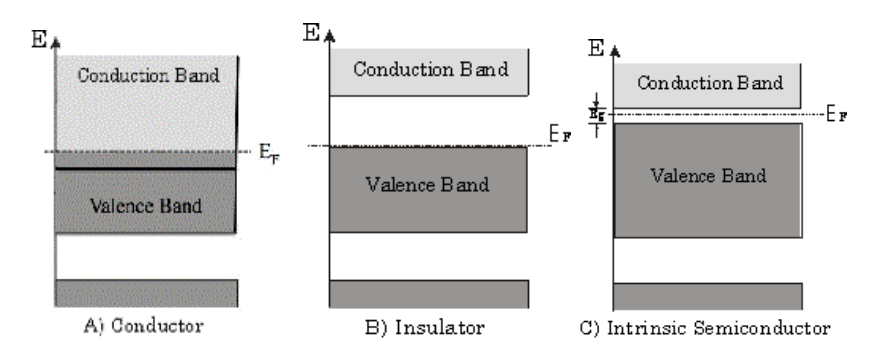
\includegraphics[scale=0.7]{images/semiconductor-band-graph.png}
		\caption{Diagram showing the different valence and conduction band configurations for (A) a
			conductor, (B) an insulator, and (C) a semiconductor. The semiconductor here is labeled
		\textit{intrinsic}, meaning that there are zero impurities in the semiconductor crystal.}   
		\label{energy-band}
	\end{figure}

	\subsection{Doping}
	\label{doping}

	The small band gap of semiconductors lends itself very well to a process called \textit{doping}, which
	allows us to alter the band gap energy. We do this by introducing some selected impurities into the
	semiconductor, which has the effect of either increasing the energy of the valence band or decreasing the
	energy of the conduction band. The type of effect we receive is determined by the kind of dopant atom we
	use: if we use an atom with an ionization energy lower than that of the intrinsic material, then we lower
	the conduction band, since the electron in this atom excites to the conduction band at a lower energy. By
	contrast, if we use an atom with a high ionization energy, then electrons will bind to this atom at a
	higher energy, thus increasing the energy of the valence band. The former case is also known as "electron
	doping" and is called an n-type semiconductor, and the latter is called "hole doping" and called a p-type
	semiconductor.  

	One characteristic effect of this doping is that it splits the semiconductor behavior into two regimes
	based on temperature. To see why, consider a semiconductor doped with an electron with lower ionization
	energy.\footnote{the exact reverse of this argument is the case where you hole dope instead of electron
	dope.} At temperatures where \( k_BT \sim E_g \) of the intrinsic material, both the doped electrons and
	the intrinsic electrons can excite to the conduction band. 
	Since the electrons from the intrinsic
	material participate in conduction, this regime is often called the \textit{intrinsic regime}.  
	However, due to the lower ionization energy of
	the doped atoms, there exists a temperature range in which only the doped electrons can promote to the
	conduction band, which is called the \textit{extrinsic regime}. 
	The "phase transition" between these two
	regimes is completely determined by the properties of the doping atom we use, and the physics of the
	phase transition is complex, so we will make simplifications of the physics here in our analysis. 
	Figure \ref{regime-graph}
	shows the transition between what the extrinsic and intrinsic regime looks like in terms of electron
	concentration (in essence, the number of electrons participating in conduction). 
	Note that there is also the regime of partial ionization on the graph, but this regime
	will not be relevant for us in this lab.  

	\begin{figure}
		\centering
		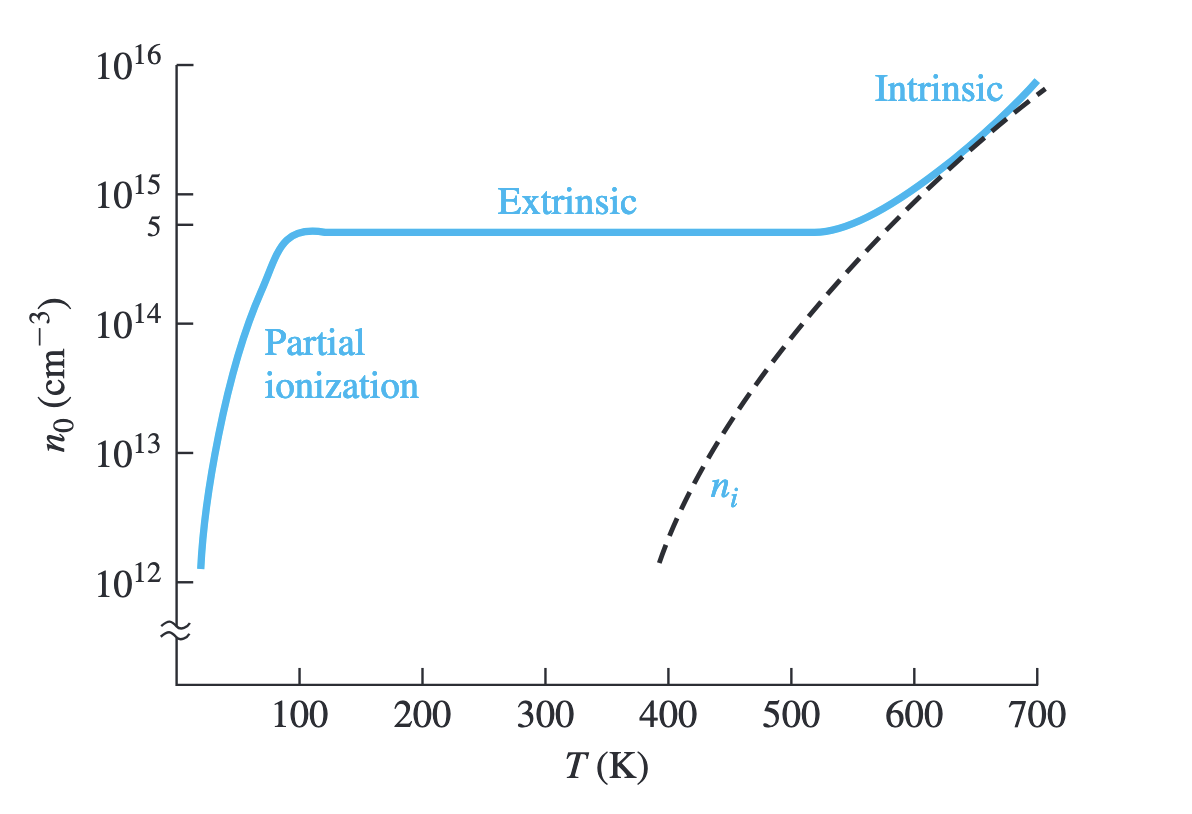
\includegraphics[scale=0.5]{images/regime-graph.png}
		\caption{Diagram showing the electron concentration of a semiconductor against temperature, with the different
			semiconductor regimes labeled. The objective of this figure is just to illustrate the different
			regimes we're working in, so if there's anything to take away it's that the semiconductor behaves
		very differently depending on which regime it's in. This diagram is taken from \cite{neamen}.}
		\label{regime-graph}
	\end{figure}

	\subsection{Hall Effect} 
	
	\subsubsection{One Carrier}

	Now, we turn to the Hall effect, the derivation of which we follow \cite{neamen} closely. 
	To explain this phenomenon, consider a semiconductor placed in a uniform
	magnetic field \( \mathbf{B} \). Then, we pass a current \( \mathbf{I} \) perpendicular to \( \mathbf{B} \). Then,
	because current is modeled as moving charge carriers, they will be deflected by the magnetic field,
	due to the Lorentz force \( \mathbf{F} = q (\mathbf{v} \times \mathbf{B}) \). Due to this deflection, we
	will end up with an accumulation of charge on one side of the semiconductor, which generates an electric
	field \( \mathbf{E} \). This strength of the \( \mathbf{E} \) field is exactly enough such that the net
	force on the electrons is zero. That is, 
	\begin{equation}
		\label{hall-effect}
		\mathbf{F} = q(\mathbf{E} + \mathbf{v} \times \mathbf{B}) = \mathbf{0} \implies \mathbf{E} +
		\mathbf{v} \times \mathbf{B} = \mathbf{0}
	\end{equation}
	From this formula, we can deduce that the electric field strength \( \mathbf{E} \) is dependent on \(
	\mathbf{v} \) and \( \mathbf{B} \). Here, \( \mathbf{v} \) is controlled by the current, and \( \mathbf{B}
	\) is the external magnetic field we apply. This \( \mathbf{E} \) field can also be measured via the
	relation that \( \mathbf{E} = -\nabla V \), and due to the uniformity of the \( \mathbf{E} \) field we get \( V_H
	= E_H W\), where \( W \) is the length of the semiconductor along the direction of the \( \mathbf{E}
	\) field. The polarity (or sign) of \( V_H \) is determined by whether the charge carriers are positively
	or negatively charged -- in a p-type semiconductor the charge carriers are positive, so \( V_H > 0 \),
	and the opposite is true for n-type semiconductors. 

	Other quantities can also be determined from the Hall effect. To illustrate this, first we notice that
	from equation \ref{hall-effect}, we have the equation:
	\[
		q \mathbf{E} = q (\mathbf{v}_x \times \mathbf{B}_z)
	\]
	combining this with \( V_H = E_H W \), we obtain, in terms of magnitude:
	\[
		V_H = \mathbf{v}_x W \mathbf{B}_z
	\]
	here, \( v_x  \) represents the (average) velocity of the electrons through the semiconductor; the book calls this
	the \textit{drift velocity}. Finally, the last equation we will use is the expression for the drift
	velocity in terms of the current and hole density \( p \):
	\[
		\mathbf{v}_x = \frac{\mathbf{J}_x}{ep} = \frac{\mathbf{I}_x}{(ep)(Wd)}
	\]
	To explain this formula, it is perhaps more useful to write it as \( I_x = v_x (ep)(Wd) \). \( v_x \)
	represents the drift velocity, \( ep \) is just a representation of how much charge is moving as it is a
	charge multiplied by a density, and \( Wd \) is just the dimensions of the semiconductor. Put this way,
	it should make sense why the formula for \( I_x \) is written like this:\footnote{I also want to
		acknowledge that here, I'm not writing \( I_x \) as a vector quantity as I did in the line above;
	this is because there is only one direction the current could flow in, so the direction is obvious.} 
	the current is a measure
	of how much moving charge there is, and the right hand side represents that by multiplying together a
	drift velocity and the "amount" of charge, which is a density times a volume. Finally, putting
	this together with the previous result, we end up with the first of two equations:
	\begin{equation}
		\label{vh-pos}
		V_H = \frac{\mathbf{I}_x \mathbf{B}_z}{epd}
	\end{equation}
	An analogous approach can be followed for an n-type semiconductor can also be done, where we arrive at
	the equation:
	\begin{equation}
		\label{vh-neg}
		V_H = -\frac{\mathbf{I}_x \mathbf{B}_z}{end}
	\end{equation}
	Notice the change in sign here, so \( V_H \) is negative when we have an n-type semiconductor, and
	positive when we have a p-type. This difference in \( V_H \) is what will allow us to determine the type
	of semiconductor we deal with in the experiment. With these equations, we can also calculate a quantity
	called the \textit{Hall coefficient} \( R_H \):
	\begin{equation}
		\label{rh}
		R_H = \frac{E_H}{J_x B_z} = \begin{cases}
			\dfrac{1}{en} & \text{n-type}\\
			-\dfrac{1}{ep} & \text{p-type}
		\end{cases}
	\end{equation}
	Intuitively, this Hall coefficient is effectively a measure of the strength of the generated electric
	field \( \mathbf{E} \) relative to the strength of the magnetic field that we introduce into the system.
	The Hall coefficient is something that we will be able to measure, and its sign will tell us which type
	of semiconductor we are working with. 

	\subsubsection{Multiple Carriers}
	\label{multiple-carriers}
	It should also be mentioned here that this above equation for \( R_H \) only works in the case of a
	single charge carrier, and a more complete equation is required when both positive and negative charge
	carriers are present. For this, we turn to \cite{melissinos} for a complete treatment. The first thing to 
	notice is that despite there being different charges present, there is still no current flowing in the \(
	y\) direction, so therefore there should be no current flowing along this axis. Assuming that the drift
	velocities of both positive and negative charge carriers to be the same, this relation can be expressed
	as:
	\begin{equation}
		\label{vy}
		e(\mathbf{v}_y^{+}n - \mathbf{v}_y^{-}n) = 0
	\end{equation}
	Here, \( v_y^{+} \) represents the velocity of the positive charges in the \( y \) direction, and \( v_y^{-}
	\) is the same but for negative charges. \cite{melissinos} also provides a formula for the drift velocity which we
	will make use of:
	\[
		\mathbf{v}_y = \left( \frac{1}{2} \frac{\mathbf{F}}{m}d^2 \right)\frac{1}{d}
	\]
	Now, \( \mathbf{F} \) acts on the carriers differently based on their charge. In particular, we have:
	\begin{align*}
		\mathbf{F}^{+} &= e[(\mathbf{v}_x^{+} \times \mathbf{B}) + \mathbf{E}_y] \\ 
		\mathbf{F}^{-} &= -e[(\mathbf{v}_x^{-} \times \mathbf{B}) + \mathbf{E}_y] 
	\end{align*}
	Here, we introduce a new term, called the \textit{carrier mobility}. Intuitively, the carrier mobility
	represents how fast a charge carrier can make its way through a material when under the presence of an
	electric field, and it is defined as:
	\[
		\mu = \frac{v}{E}
	\]
	This carrier mobility is also a fundamental property of the semiconductor, and is one of the quantities
	we are interested in calculating for our sample. Here, because we have two different charges, we will
	consider the positive and negative carriers separately, and using this new relation between \(
	\mathbf{v}_x \) and \( \mu \), we can combine this with equation \ref{vy} to arrive at the following
	relationships for \( \mathbf{v}_x^{+} \) and \( \mathbf{v}_x^{-} \):
	\begin{align*}
		\mathbf{v}_x^{+} &= \mu_p(\mu_p \mathbf{E}_x \mathbf{B} + \mathbf{E}_y)\\
		\mathbf{v}_x^{-} &= \mu_n(\mu_n \mathbf{E}_x \mathbf{B} - \mathbf{E}_y)
	\end{align*}
	and finally, plugging this back into equation \ref{vy}, we finally get the following relationship between
	\( \mathbf{E}_y \) and \( \mathbf{E}_x \):
	\[
		\mathbf{E}_y = \mathbf{E}_x B \frac{\mu_p^2 p - \mu_n^2 n}{\mu_p p + \mu_n n}
	\]
	Finally, since we have a formula for \( R_H \) from equation \ref{rh}, we may write:
	\[
		R_H = \frac{\mathbf{E}_y}{\sigma \mathbf{E}_x \mathbf{B}} = \frac{\mu_p^2 p - \mu_n^2 n}{e(\mu_p p +
		\mu_n n)^2}
	\]
	which is the "complete" form for \( R_H \) given two carriers present. Note that this equation does
	actually become \ref{rh} if we set either \( p \) or \( n \) to zero, as expected. The \( \sigma \) term
	represents the \textit{conductivity}, which is related to the resistivity by \( \sigma = 1 / \rho \);
	this will be one of the values we are interested in.
	\subsection{The Van Der Pauw Technique}
	In our experiment, the main technique we will employ to determine the semiconductor characteristics is
	called the \textit{Van Der Pauw Technique}. This technique, popularized by Leo van der Pauw in 1958,
	allows us to measure characteristics such as the resistivity and the carrier mobilities in a
	semiconductor. This technique is also very powerful, as it can be used on a semiconductor of arbitrary
	shape, provided that the following criteria are satisfied:
	\begin{enumerate}[label=\arabic*.]
		\item The contacts are at the circumference of the sample.
		\item The contacts are sufficiently small.
		\item The sample is an even thickness.
		\item The sample does not have holes (i.e. the sample is a slab with no holes in it; this isn't
			referring to electron holes).
	\end{enumerate}
	\cite{vdp}. 
	In our experiment, the semiconductor is a square shape of even thickness, with small leads placed on the
	corners of the shape (see figure \ref{setup-2}), 
	so in this case all four of these conditions are actually satisfied. 

	% expand on what R_ABCD actually means 
	When these conditions are satisfied, then the Van der Pauw theorem says that if we measure the voltage and
	current at these points \( A, B, C, D \), then we can find resistances \( R_{AB, DC} \) and \( R_{AD, BC}
	\) (more on how to do this later), and we have the following relation between these two quantities:
	\[
		\exp\left( -\frac{\pi d}{\rho}R_{AB, DC} \right) + \exp\left( -\frac{\pi d}{\rho}R_{AD, BC} \right) =
		1
	\]
	This equation can then be solved for \( \rho \), which yields the following form:
	\[
		\rho = \frac{\pi d}{\ln 2} \frac{(R_{AB, DC} + R_{AD, BC})}{2} \cdot f\left( \frac{R_{AB, DC}}{R_{AD,
		BC}}\right)
	\]
	The function \( f(x) \) is a function which satisfies the relation:
	\[
		\frac{R_{AB, DC} - R_{AD, BC}}{R_{AB, DC} + R_{AD, BC}} = f \cosh^{-1}\left( \frac{\exp(\ln 2 / f)}{2} \right)
	\] 
	This \( f \) is called the \textit{correlation factor}, and it is a function only of the ratio of
	resistances \( R_{AB, DC} \) and \( R_{AD, BC} \). There are many ways we can approximate \( f \); van
	der Pauw himself suggested the following approximation that applies when \( R_{AB, DC} \approx R_{AD,
	BC}\):
	\begin{equation}
		\label{vdp-1}
		f_1 \approx 1 - \left( \frac{R_{AB, CD} - R_{BC, DA}}{R_{AB, CD} + R_{BC, DA}} \right)^2 \frac{\ln
		2}{2} - \left( \frac{R_{AB, CD} - R_{BC, DA}}{R_{AB, CD} + R_{BC, DA}} \right)^{4} \left( \frac{(\ln
		2)^2}{4} - \frac{(\ln 2)^3}{12} \right)
	\end{equation}
	While \( R_{AB, DC} \approx R_{AD, BC} \) in our experiment, we will instead use a simpler approximation
	for \( f \), given to us by \cite{lab-manual}:
	\begin{equation}
		\label{vdp-2}
		f_2(x) = \frac{1}{\cosh(\ln x / 2.403)}
	\end{equation}
	which is good enough. To illustrate how good of an approximation this is, figure \ref{vdp-compare} shows the plots
	of \( f_1(x) \) and \( f_2(x) \), where \( f_1(x) \) is equation \ref{vdp-1} and \( f_2(x) \) is
	\ref{vdp-2}. As shown in the figure, the approximations are very good for \( x \)-values up to about \( x
	\approx 4\), which is exactly the regime that we will be working in. The approximation is poor past \( x
	= 10\), but this isn't a regime we should care about at all because neither \( f_1 \) nor \( f_2 \) are
	actually meant to approximate the analytically solved \( f \) in these regimes. 

	\begin{figure}
		\centering
		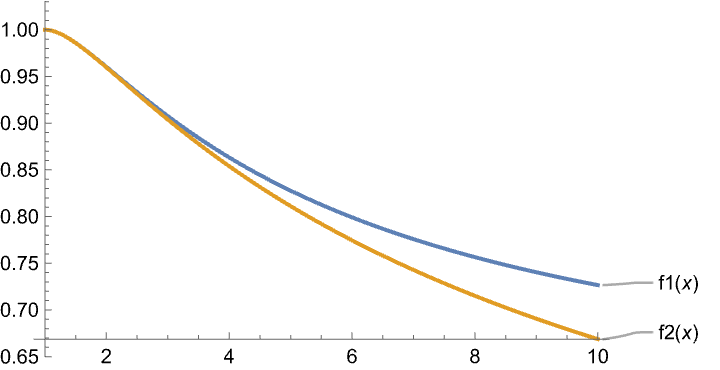
\includegraphics[scale=0.6]{images/f-graph.png}
		\caption{Comparison of the function \( f \) provided by Van der Pauw and the function \( f \) we will
			use in our approximation. While the approximation does get significantly worse past \( x = 10 \),
		our ratios (\( x \)-values) do not exist within that regime so this is a valid approximation.} 
		\label{vdp-compare}
	\end{figure}
	
	With the resistivity determined, we can then move on to determining the carrier mobilities, using the
	relation:
	\begin{equation}
		\label{mobility}
		\frac{1}{\rho} = e \left( n \mu_n + p \mu_p \right)
	\end{equation} 
	where \( \mu_n \) and \( \mu_p \) are the electron and hole densities, respectively. With this
	determined, we now have full information about the semiconductor in the sample, which is what we
	ultimately set out to determine.   

	\section{Experimental Procedure}
	Now, with the theory out of the way, we move on to the experimental procedure. We will split this section
	into two portions: first, we will explain the setup containing the semiconductor chip, and then we will
	discuss the surrounding apparatus separately. 

	To begin, figure \ref{setup-1} shows the semiconductor chip and the surrounding apparatus. On the left, there is
	an opening where we will pour in liquid nitrogen to cool the entire apparatus down. This cooling is
	transferred to the semiconductor via a copper rod, as shown in the figure. We place a brass intermediary
	here to control how quickly the sample cools down -- we want to take measurements at varying
	temperatures, so it makes sense to not want the temperature to vary too fast. On the right side, we have
	the germanium crystal (our semiconductor), surrounded by four leads from which we will make voltage and
	current measurements. We also have a temperature diode placed next to the crystal, from which we will
	take temperature measurements. Finally, there is a 50W heater, which we will use to slowly heat the
	sample and take measurements over a wide range of temperatures.        

	\begin{figure}
		\centering
		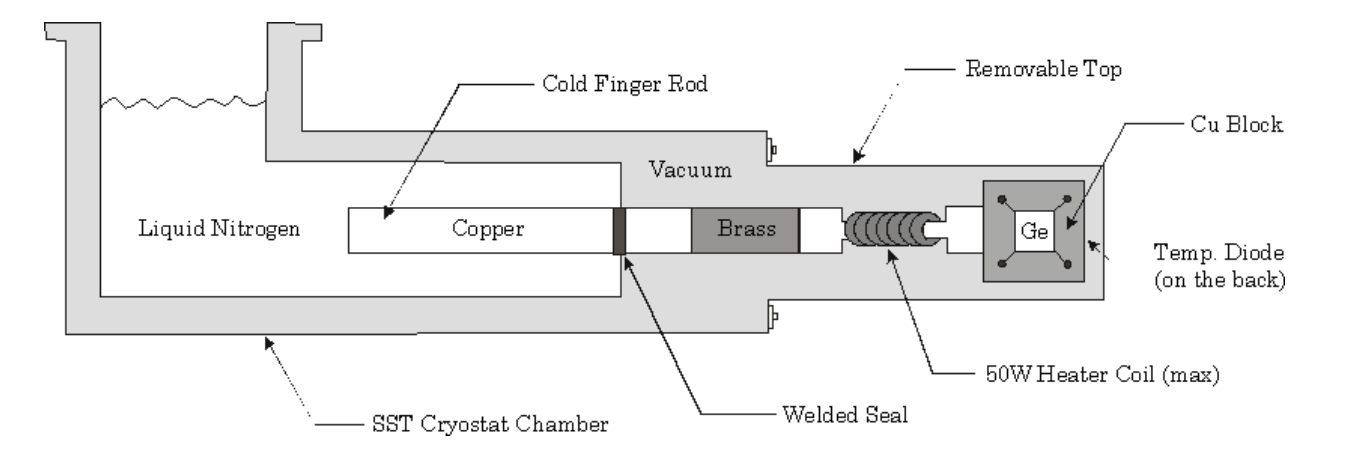
\includegraphics[scale=0.5]{images/setup-1.png}
		\caption{Block diagram of the central apparatus.}
		\label{setup-1}
	\end{figure}

	Figure \ref{setup-3} shows a block diagram setup of the surrounding apparatus. The primary elements that
	we care about in this diagram are the electromagnet (a Helmholtz coil), which generates the uniform
	\( \mathbf{B} \) field in the experiment, and the various meters in the bottom left. The meters record
	valuable information: the strength of \( \mathbf{B} \) field, the voltage and current measurements, as
	well as the temperature. All of this information is fed into the DAQ box, which is then fed into the
	computer and displayed on the \texttt{control\_program.vi} LabVIEW program. From here, we then export
	the data to a \texttt{.csv} file, from which it is ready to be analyzed. 

	\begin{figure}
		\centering
		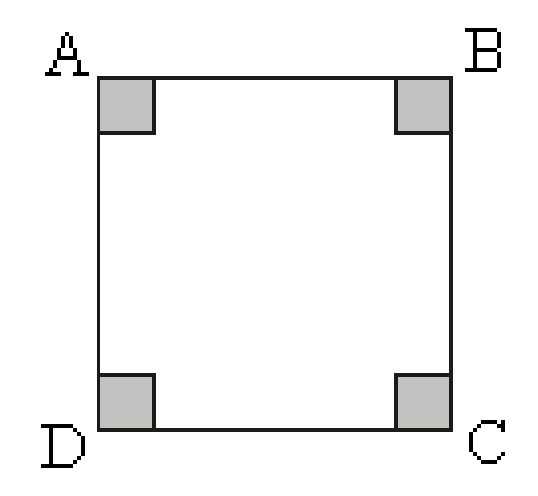
\includegraphics[scale=0.5]{images/setup-2.png}
		\caption{Schematic of the semiconductor chip, with leads placed at points \( A, B, C, D \) to perform
		voltage and current measurements.}
		\label{setup-2}
	\end{figure}
	Our experimental procedure for this experiment is relatively straightforward. First, we start the water
	cooling pumps, and turn on the 
	vacuum pump\footnote{The reason for a pump is to prevent the germanium crystal from oxidizing; it has no
	measurable effect on the measurements themselves.} and wait for the pressure in the chamber to below 
	90 millitorr. At this
	point, we begin pouring LN2 to the left side, and wait until the temperature drops to around 
	240 K. At this point, we pour the LN2 a second time, which will cool the sample to a temperature of
	around 90 K. While the apparatus is cooling, we turn on the other requisite equipment: the power supply
	to the heater, the Helmholtz coils, and also turn on the computer to record the measured data. This data
	is automatically collected for us via the "gold box", so all we have to do at this point is to just wait
	for all the data to be collected and upload it as a \texttt{.csv} file. 

	While pouring LN2 is the only manual thing we do in terms of data collection, we should still become
	familiar with what the apparatus is doing to perform its measurements. From what we could gather, the
	following steps are carried out for a given temperature reading:
	\begin{enumerate}[label = \arabic*.]
		\item Record the temperature of the semiconductor.
		\item With the magnetic field switched on (current flowing through the Helmholtz coils), 
			record the strength of the magnetic field using the 450
			Gaussmeter.
		\item Using the probes attached to the semiconductor, send a current along \( AB, AD, AC, BD \) and
			also along the reverse directions.  
		\item For each current measurement, measure the voltage along the two probes that are not used to
			send current (i.e. if current is sent along \( AB \), then we measure voltage along \( CD \), and so on).
		\item Reverse the polarity of the magnetic field (amounts to switching the direction of current) and
			repeat steps 2-4. 
		\item Once the positive and negative polarity data is taken, we then take a "zero field" measurement,
			by effectively running a vanishingly small current through the Helmholtz coils so that we
			approximate 0 G.  
	\end{enumerate}
	This process is done repeatedly for different temperature values, so we have data over a range of
	95 K to approximately 350 K. Finally, we repeat this entire process different values of current, six of
	them to be exact. For some of our datasets, unfortunately the lab period ended just before the data could
	finish collecting, so some of our datasets stopped at around 330 K, but as we will see this won't
	affect the results that much. Now with the theory and procedure complete, we are ready to move on to the
	analysis. 

	\section{Analysis}
	Now we move on to the analysis of the report. Above, we detailed how we took measurements for different
	current values, so this analysis section will detail the calculations performed for a single current
	dataset (30uA), then we will present our findings over all current values at the end. We will also go in order
	of the lab manual, detailing the things that are required in this report. 

	\subsection{Resistivity and Hall Coefficient at Room Temperature}
	This section is relatively simple: directly from our measurements, we can use the Van der Pauw method and
	equation \ref{vdp-1} to determine the resistivity for all temperatures. Then, we can then take its
	reciprocal and compute the conductivity as a function of temperature as well. This is then plotted
	against inverse temperature, and shown in figure \ref{rho-plot}. One thing to notice about the plot is
	that the resistivity is just ever so slightly different for positive and negative field; this is a
	phenomenon we observe but we don't have a concrete explanation for. One leading theory we have is that
	this has to do with Earth's ambient magnetic field, but we do not know how to confirm or reject this
	hypothesis.   
	\begin{figure}
		\centering
		\begin{subfigure}{0.45\textwidth}
			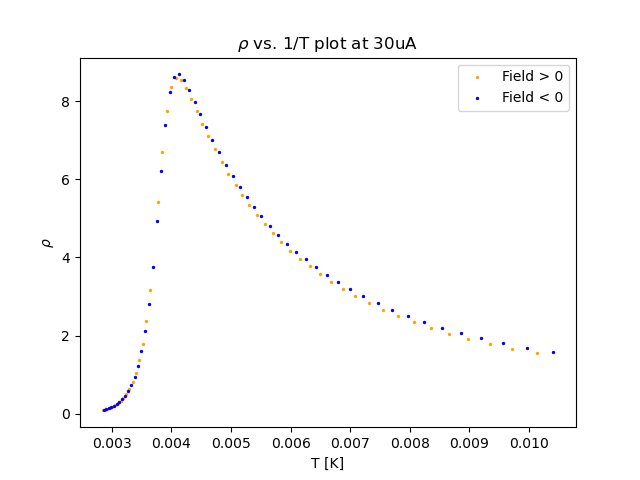
\includegraphics[width = \textwidth]{images/30uA-rho-plot1.png}
			\caption{}
		\end{subfigure}
		\begin{subfigure}{0.45\textwidth}
			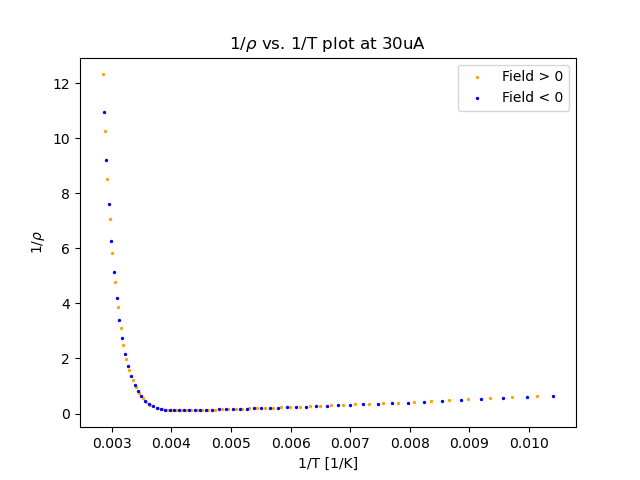
\includegraphics[width = \textwidth]{images/30uA-rho-plot2.png}	
			\caption{}
		\end{subfigure}
		\caption{Plot of (a) resistivity and (b) conductivity versus inverse temperature. Note that these
			relationships do make sense intuitively: the conductivity increases as temperature decreases (or
		equivalently, as \( 1 / T \) decreases, so this is a good indication that our plots are accurate.}
		\label{rho-plot}
	\end{figure}

	The plot for the Hall coefficient is more relevant for the next section, so we will discuss it further
	there. The plot is given in figure \ref{30uA-rh}. 

	\subsection{Semiconductor Type}
	Now, with the theory established, we are ready to move on to the central focus of this report. To begin,
	it is beneficial to go over all the data we collect, so that the steps taken in the analysis are clear.
	The quantities we recorded throughout the experiment were the temperature, the surrounding \( B \) field
	in Gauss, and the voltage and current measurements from each pair of leads \( A, B, C, D \). To compute
	the resistivity, we will use the measurements that come from sending current through adjacent points, and
	for the Hall voltage we will compute from the current being driven across non-adjacent points.  

	To begin,
	the first quantity we should calculate is the Hall coefficient \( R_H \), because calculating it will
	allow us to determine crucial information about what kind of semiconductor we are dealing with. To see
	why this is, consider what happens when we plugin equation \ref{rh} into equation \ref{vh-pos} or
	\ref{vh-neg}. In either case, working out the signs, we the following relation between \( R_H \) and \(
	V_H \):
	\[
		V_H = -\frac{R_H I_x B_z}{d}
	\]
	Since we measure \( V_H \), \( I_x \) and \( B_z \), then plotting \( V_H \) against \( R_H \) will give
	us the sign of \( R_H \). Specifically, from this equation we can deduce that the slope is given by:
	\[
		m = - \frac{I_x B_z}{d} \sgn(R_H)
	\]
	where \( \sgn(\cdot) \) is the sign function. So, for \( B_z \) of a given sign, the sign of the slope
	will allow us to determine the sign of \( R_H \), and hence whether \( R_H \) is given by \( 1 / en \)
	or \( -1 / ep \). In the latter case, we know we have a p-type, and in the former we conclude it's an
	n-type. Figure \ref{v-vs-rh} shows the resulting plot, where we color-code the points based on the sign of the
	surrounding field. As shown in the figure, points with a positive \( B_z \) exhibit a positive slope, so
	hence \( R_H \) is negative, and thus we have a p-type semiconductor. In addition, as explained in
	appendix \ref{B}, another way to confirm this is to plot \( R_H \) as a function of temperature: if the
	sign of \( R_H \) flips, then this is an indication of a p-type semiconductor. This is precisely what we
	observe (figure \ref{30uA-rh}), so this further confirms the fact that we are indeed working with a p-type
	semiconductor. Note that while we do plot \( R_H \) against inverse temperature in figure \ref{30uA-rh},
	the change in sign should still exist; plotting against inverse temperature does not change this fact.   

	\begin{figure}
		\centering
		\begin{subfigure}{0.45\textwidth}
			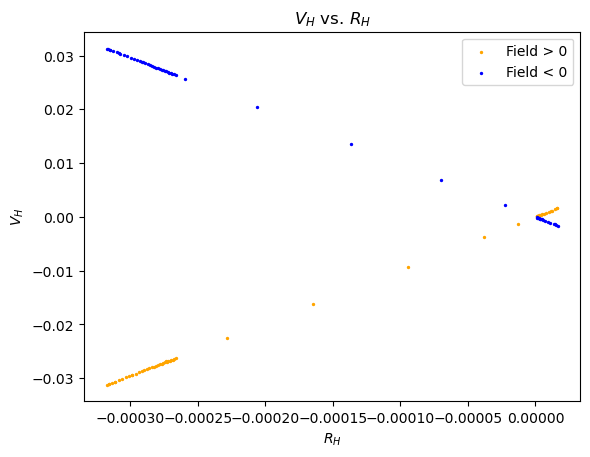
\includegraphics[width=\textwidth]{images/v-vs-rh.png}
			\caption{}
			\label{v-vs-rh}
		\end{subfigure}
		\begin{subfigure}{0.47\textwidth}
			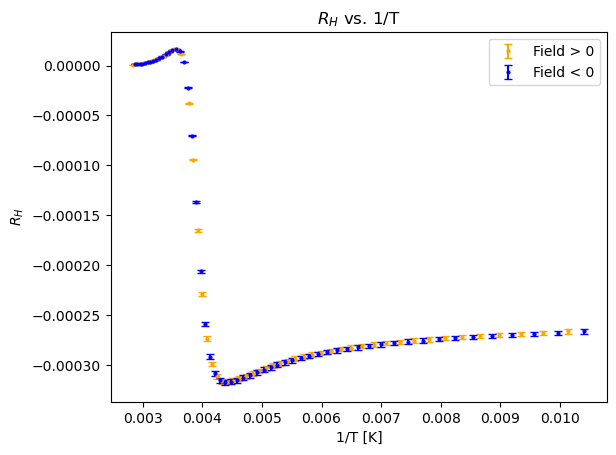
\includegraphics[width=\textwidth]{images/30uA-rh-plot2.png}
			\caption{}
			\label{30uA-rh}
		\end{subfigure}
		\caption{Two different ways determining the identity of the semiconductor. (a) A plot of the Hall
			voltage against the Hall coefficient, \( R_H \). The positive slope of the line for positive \(
			B_z \) allows us to conclude that the semiconductor is a p-type. (b) A plot of the Hall
			coefficient \( R_H \) against inverse temperature, notice the flip in sign at around \( 1 / T
		\approx 0.0035\), and the presence of a sign flip is indicative of a p-type semiconductor.}    
	\end{figure}

	\subsection{Carrier Mobilities}

	\subsubsection{Calculating the hole mobility}
	The next thing we calculate is the carrier mobilities of the semiconductor. We do this via equation
	\ref{mobility}, except in this equation we have both \( \mu_n \) and \( \mu_p \) to determine. In order
	to simplify this, we first consider the semiconductor in the extrinsic regime. In this regime, the
	intrinsic electrons from the germanium crystal don't have enough energy to be promoted to the conduction
	band; only the doped atoms can because of their lower ionization energy. Therefore, in the extrinsic
	regime, we have \( n = 0 \), and thus our equation simplifies to:
	\begin{equation}
		\label{carrier-extrinsic}
		\frac{1}{\rho} = e p \mu_p = -\frac{\mu_p}{R_H}
	\end{equation}
	which is a much simpler equation to calculate. Since we know \( R_H \) from earlier, we can use it and
	equation \ref{rh} to solve for \( p \), and we can also use the Van der Pauw method to determine \( \rho
	\), using equation \ref{vdp-1} as our choice for \( f \). With these two quantities determined, we now
	have \( \mu_p \) in the extrinsic regime. According to \cite{neamen}, the carrier mobility has a nice scaling
	with temperature, it scales as \( \mu_p \propto T^{-\alpha} \), so we can plot \( \mu_p \) versus \( T \) and
	perform a least-squares fit to experimentally determine \( n \). This least squares fit is shown in
	figure \ref{mu-vs-T}, and we get an \( n \)-value of \( n = -1.883 \pm 0.0012 \) for a current \( I_x =
	\SI{15}{\micro\ampere} \), with a table showing the \( \alpha \) fit values for all currents displayed in
	table \ref{alpha-fit}. Taking the average of all \( \alpha \) values, we get a mean value of \( \alpha = -1.88 \pm
	0.0009 \). 
	According to \cite{neamen}, first-order scattering theory predicts that \( \alpha =
	-\frac{3}{2} \), but in most experimental circumstances this \( T^{- 3 / 2} \) relationship is never
	observed \cite{melissinos}. Thus, it's really hard to say whether our values are accurate, but at the very minimum,
	our values are consistent (see table \ref{alpha-fit}), and this alone is strong evidence for the fact
	that our fitted dependence is likely accurate. 
	
	\begin{table}
		\centering
		\def\arraystretch{1.75}
		\begin{tabular}{|c|c|c|}
			\hline
			\textbf{Current ($\mu$A)} & \textbf{$\alpha$} & \textbf{$T_0$} \\ \hline
			5                         & $-1.8790 \pm 0.0009$                   & 269.813        \\ \hline
			15                        & $-1.8918 \pm 0.0017$                   & 270.259        \\ \hline
			30                        & $-1.8832 \pm 0.0011$                   & 270.525        \\ \hline
			45                        & $-1.8744 \pm 0.0006$                   & 270.408        \\ \hline
			60                        & $-1.8792 \pm 0.0009$                   & 269.925        \\ \hline
			75                        & $-1.8802 \pm 0.0010$                   & 269.785        \\ \hline
			90                        & $-1.8805 \pm 0.0009$                   & 270.642        \\ \hline
		\end{tabular}
		\caption{Fit values for \( \alpha \) for all current values.}
		\label{alpha-fit}
	\end{table}

	\begin{figure}
		\centering
		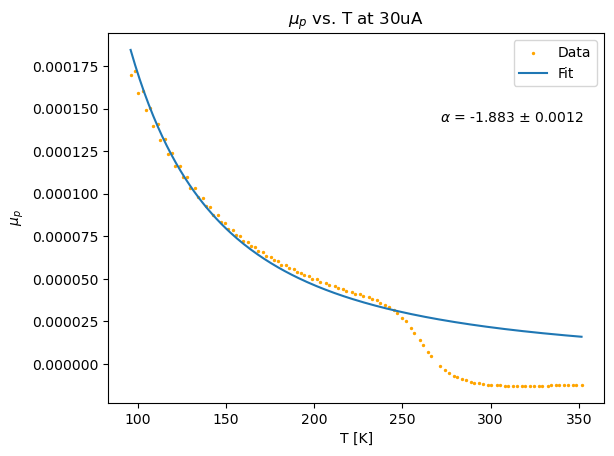
\includegraphics[scale=0.7]{images/30uA-mu-plot.png}
		\caption{Plot of the hole mobility against temperature, with a fitted constant of \( \alpha = -1.883
			\pm 0.0012 \). Notice that the exponential fit clearly fails
			to account for the transition between the extrinsic and intrinsic regimes of the semiconductor,
			as expected. However, in the extrinsic regime, the decaying exponential plot fits the data
		relatively well.}   
		\label{mu-vs-T}
	\end{figure}

	Looking at figure \ref{mu-vs-T} more closely, we see that the decaying exponential relationship becomes
	inaccurate at around 240 K, and this signals the transition between the extrinsic and intrinsic regimes
	of the semiconductor, as \( n \) no longer becomes negligible and thus equation \ref{carrier-extrinsic}
	no longer holds. However, the from this fit we determined \( \mu_p \) for all values of \( T \), which
	will be useful in the next section.  
	% write theory on carrier mobility vs. temperature 

	\subsubsection{Calculating the electron mobility}
	Now with the hole mobility determined, it is now possible to determine the electron mobility. For this
	section, we will follow the analysis method provided in \cite{melissinos}; here we will only highlight the relevant
	equations we need for the analysis, a more detailed explanation can be found in the appendix.

	The key to determining the electron mobility is to look closely at the temperature where \( R_H = 0 \),
	we will denote this as \( T_0 \). This temperature is special because it provides some special
	relationships between quantities we want to calculate. In particular, \cite{melissinos} mentions the following
	approach: using our fitted value of \( \mu_p \), we can use equation \ref{carrier-extrinsic} to
	\textit{extrapolate} the conductivity to the point \( T = T_0 \) to get \( \sigma_e(T = T_0) \), 
	and from the Van der Pauw method we can
	experimentally determine the conductivity at \( T_0 \) using 
	\( \sigma_0 = 1 / \rho(T = T_0)\). Then, comparing the two values,
	we then have the following relationship:
	\begin{equation}
		\label{sigma}
		\frac{\sigma_0}{\sigma_e} = \frac{b}{b - 1}
	\end{equation}
	where \( b = \mu_n / \mu_p \), the ratio of carrier mobilities. We can experimentally calculate this
	ratio \( \sigma_0 / \sigma_e \), which means that for this equation we can solve for \( b \), and thus we
	can now solve for \( \mu_n \) since we already have \( \mu_p \). The combined plot of \( \mu_p \) and \(
	\mu_n\) along with their exponential fits are shown in figure \ref{double-plot}. As demonstrated in the
	plot, the exponential fit becomes significantly worse past \( T \approx 240 \) K, but this is to be
	expected, since our formula we used to compute \( \mu \) experimentally only holds when there's 
	one carrier present. So,
	it is natural that the data does not match the plot, but in this case the plot is to be trusted instead.

	\begin{figure}
		\centering
		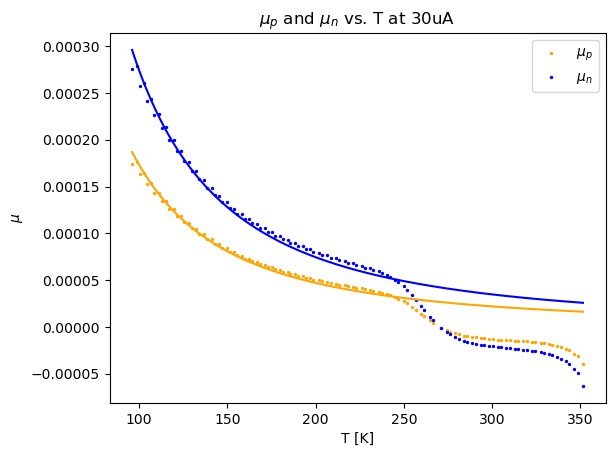
\includegraphics[scale=0.75]{images/30uA-double-mu-plot.png}
		\caption{Plot of \( \mu_p \) and \( \mu_n \) as a function of temperature, along with their fitted
			decaying exponential curves. Again, notice that the fit does not work in the extrinsic regime, which
		makes sense since this exponential is only true in the case where there is one carrier present.}
		\label{double-plot}
	\end{figure}

	\subsection{Calculating the Electron and Hole Densities}
	Now we move on to calculating the electron and hole densities. To do this, we will continue following the
	analysis given in \cite{melissinos}. First, we will make the following assumption about the behavior of our
	semiconductor: within the intrinsic and extrinsic regimes, the semiconductor behaves ideally, so 
	in the extrinsic regime there are \textit{zero} intrinsic carriers participating, and
	\textit{all} dopant carriers participate.
	Given this, then we may write that \( p \) is equal to the total number of
	dopant atoms, or \( p = N_a \). Likewise, the number of negative carriers \( n \) we will set to zero in
	this regime. In the intrinsic regime, the intrinsic carriers do participate, so let \( n = N \). Because
	the electrons and holes now come in pairs, then there is a matching hole for every electron, so \( p =
	N_a + N \). Using these two relations, \cite{melissinos} shows that we have:\footnote{It should also be obvious that 
		this is indeed a simplification on the true physics of the system -- from this analysis, the result we obtain
		is that \( n \) and \( p \) are constants in both the extrinsic and intrinsic regime, but this is at
		least somewhat untrue since from statistical mechanics, there should still be some atoms that don't
		have the appropriate amount of energy to promote to the conduction band. We theorize that the reason
		we can still make this assumption is because we are using extremely small currents, on the order of
		microamps. Therefore, the number of carriers required to facilitate such a current immediately
	saturates after the phase transition.} 
	\begin{equation}
		\label{electron-density}
		n = \frac{N_a}{b^2 - 1}
	\end{equation}
	where \( b \) is the same ratio of mobilities as in \ref{sigma}. 
	So, in summary, the following is what we need to do to determine the densities in the extrinsic regime:
	we first calculate \( p \) in the extrinsic regime to get \( N_a \), and combine this with our value of
	\( b \) and equation \ref{electron-density} to determine \( n \). With this relation, we now have the
	electron and hole densities in both the intrinsic and extrinsic regimes, and we've determined all the
	relevant quantities in the semiconductor. The \( n \) and \( p \) values in both regimes, for all current
	values are given in table \ref{densities}.  

	\begin{table}[]
		\centering
		\def\arraystretch{1.75}
		\begin{tabular}{|c|cc|cc|}
			\hline
			\multicolumn{1}{|c|}{\multirow{2}{*}{\textbf{Current ($\mu$A)}}} & \multicolumn{2}{c|}{\textbf{Extrinsic}}                           & \multicolumn{2}{c|}{\textbf{Intrinsic}}                           \\ \cline{2-5} 
			\multicolumn{1}{|c|}{}                                           & \multicolumn{1}{c|}{\textbf{p}} & \multicolumn{1}{c|}{\textbf{n}} & \multicolumn{1}{c|}{\textbf{p}} & \multicolumn{1}{c|}{\textbf{n}} \\ \hline
			5                                                                & \multicolumn{1}{l|}{2.2082e+22} & 0                               & \multicolumn{1}{l|}{3.5670e+22} & 1.3587e+22                      \\ \hline
			15                                                               & \multicolumn{1}{l|}{2.2084e+22} & 0                               & \multicolumn{1}{l|}{3.8055e+22} & 1.5970e+22                      \\ \hline
			30                                                               & \multicolumn{1}{l|}{2.2149e+22} & 0                               & \multicolumn{1}{l|}{3.7278e+22} & 1.5129e+22                      \\ \hline
			45                                                               & \multicolumn{1}{l|}{2.1752e+22} & 0                               & \multicolumn{1}{l|}{3.5300e+22} & 1.3547e+22                      \\ \hline
			60                                                               & \multicolumn{1}{l|}{2.2030e+22} & 0                               & \multicolumn{1}{l|}{3.5687e+22} & 1.3657e+22                      \\ \hline
			75                                                               & \multicolumn{1}{l|}{2.2006e+22} & 0                               & \multicolumn{1}{l|}{3.5536e+22} & 1.3530e+22                      \\ \hline
			90                                                               & \multicolumn{1}{l|}{2.2183e+22} & 0                               & \multicolumn{1}{l|}{3.6632e+22} & 1.4449e+22                      \\ \hline
		\end{tabular}
		\caption{Table of the positive and negative charge carrier densities in the extrinsic and intrinsic
			regimes. In the extrinsic regime, we have \( n = 0 \), and in the intrinsic regime we have \( p = N_a
			+ n\), where \( N_a \) is the value for \( p \) in the extrinsic regime, and \( n \) is the electron
		carrier density.}
		\label{densities}
	\end{table}

	% include a section on conductivity and resistivity
	\subsection{Hall Mobilities and Zero Field}
	The last two quantities that we want to calculate is the Hall mobility and also the resistance at zero
	field. The Hall mobility is really just another measure of the carrier mobility, and is computed as \(
	\mu_H = R_H \sigma \). We have both these values on the right from earlier already, so we can just
	calculate it and plot it against temperature. The plot is shown in figure \ref{hall-mobility}.

	\begin{figure}
		\centering
		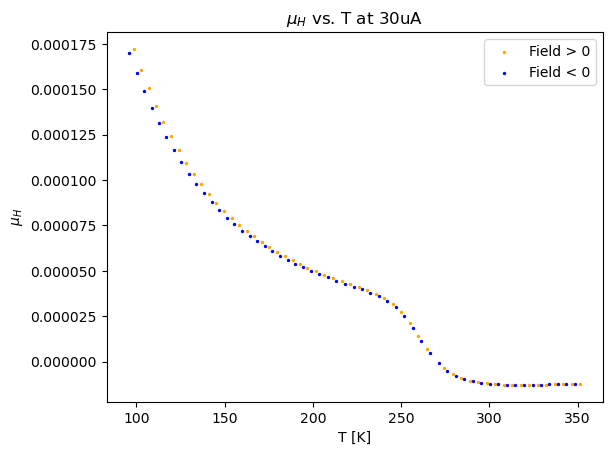
\includegraphics[scale=0.7]{images/30uA-hall-mobility.png}
		\caption{Plot of the Hall mobility \( \mu_H = R_H \cdot \sigma \) as a function of T. Note the minus
			sign is because we have a p-type semiconductor. This plot makes sense intuitively; the Hall
			mobility is just a measure of the carrier mobility, so we should expect the shape of the curve to
		look identical to that of the carrier mobilities we calculated earlier.} 
		\label{hall-mobility}	
	\end{figure}

	So far, all the plots we've been working with have involved using nonzero field measurements. The final
	quantity that we look at is the resistance and trans-resistance at zero field compared to nonzero field, 
	and the plot is shown in figure \ref{res-figure}. The resistance as measured by \( R_{AB, DC} \) at zero
	field scales in the same fashion as the resistance with nonzero field -- this is expected, since this
	quantity is used to measure the resistivity, an intrinsic property of the material that should not have a
	heavy dependence on the Hall effect. This is what we see in the plot, as we see a minor variation in the
	resistivity, but overall the scaling is unaffected.  
	The trans-resistance, however, is affected by the presence of the \( \mathbf{B} \)
	field, as it is the quantity we use to measure the Hall coefficient. Put this way, without the Hall
	effect in action, we expect the Hall coefficient \( R_H \) to equal zero, and this is reflected in our
	plots as the trans-resistance is nearly zero by comparison. It's not exactly zero however, because even
	in the case of "zero field" we are applying a very small current to the Helmholtz coils, which explains
	why the trans-resistance is not exactly zero. 
	 

	\begin{figure}
		\centering
		\begin{subfigure}{0.45\textwidth}
			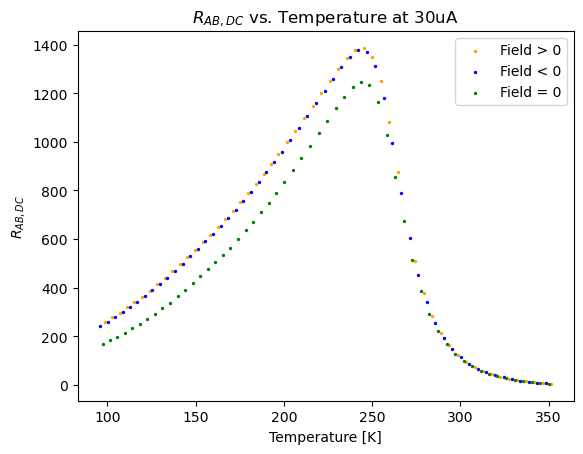
\includegraphics[width = \textwidth]{images/30uA-resistance.png}
			\caption{}
		\end{subfigure}
		\begin{subfigure}{0.45\textwidth}
			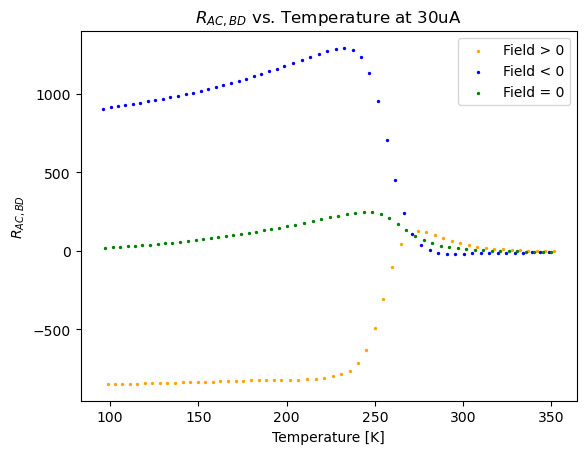
\includegraphics[width = \textwidth]{images/30uA-trans-resistance.png}
			\caption{}
		\end{subfigure}
		\caption{Plot of the (a) resistance and (b) trans-resistance of the semiconductor as a function of
			temperature. Notice that \( R_{AB, DC} \) scales and equals approximately the same values as that in
		a nonzero field, but \( R_{AC, BD} \) does not.}
		\label{res-figure}
	\end{figure}		

	\section{Reflection}
	Overall, the data we collected in this lab was a success. To be completely transparent, there wasn't
	really much that \textit{could} go wrong in our experiment anyway, because all we had to do to get the
	experiment running was pour the LN2 into the cryostat chamber and the gold box did the rest for us. As a
	result, there aren't really many sources of error for this experiment either, or rather, there isn't
	one that we can necessarily "do better" on, because the machine already does all the data collection for
	us. All we had to do was run Python code to analyze the data.    

	That said, there were a couple things out of our control which happened that affected our data, although
	not in an extremely impactful way. Just to name a few, there were were instances where despite
	making it clear that we wanted the vacuum pump to be left on overnight it was not done, so we had to
	spend lab time reinitializing the vacuum. There was also an instance where we ran out of LN2, and that
	also took a while to fix. Overall, I'd estimate that we lost about 1.5 hours of data collection time as a
	result of these delays. Luckily enough, this didn't affect our experiment quality very much, but it very
	well could have. For instance, in the 45uA trial, the first 20 data points were unreliable 
	because we forgot to turn the power supply to the coils on; luckily this didn't really affect our data as
	the solution was just to remove these points in our analysis, but in the ideal case we would have
	re-taken this dataset if we had the time. 

	That said, this experiment was still a lot of fun to do, especially when all the data analysis worked
	out. To summarize, we successfully used the Hall effect in semiconductors to learn about the properties
	of the material indirectly, using the Van der Pauw technique and some clever math. First, we were able to
	determine the type of semiconductor from the Hall coefficient, then, through some crucial assumptions, 
	we were able to determine quantities
	such as the electron and hole densities and mobilities for both the extrinsic and intrinsic regime.
	Figuring out \textit{what} to do for the analysis was definitely the hard part of this lab, but I did
	enjoy reading through different papers and gathering together what they were all saying so that I could
	formulate the logic myself -- after all, this is what doing research kind of boils down to. What's more
	interesting is the fact that even in such a simple system there are still things we don't know: for
	instance, what is the true scaling for the mobility in terms of temperature? What is the true model that
	characterizes the transition region between extrinsic and intrinsic? The fact that such a simple system
	can exhibit such complex behavior is incredibly interesting to me, and it's what made this lab so fun to
	investigate for me. 

	\nocite{*}
	\printbibliography


	\newpage
	\appendix
	\section{Figures}
	\begin{figure}[h]
		\centering
		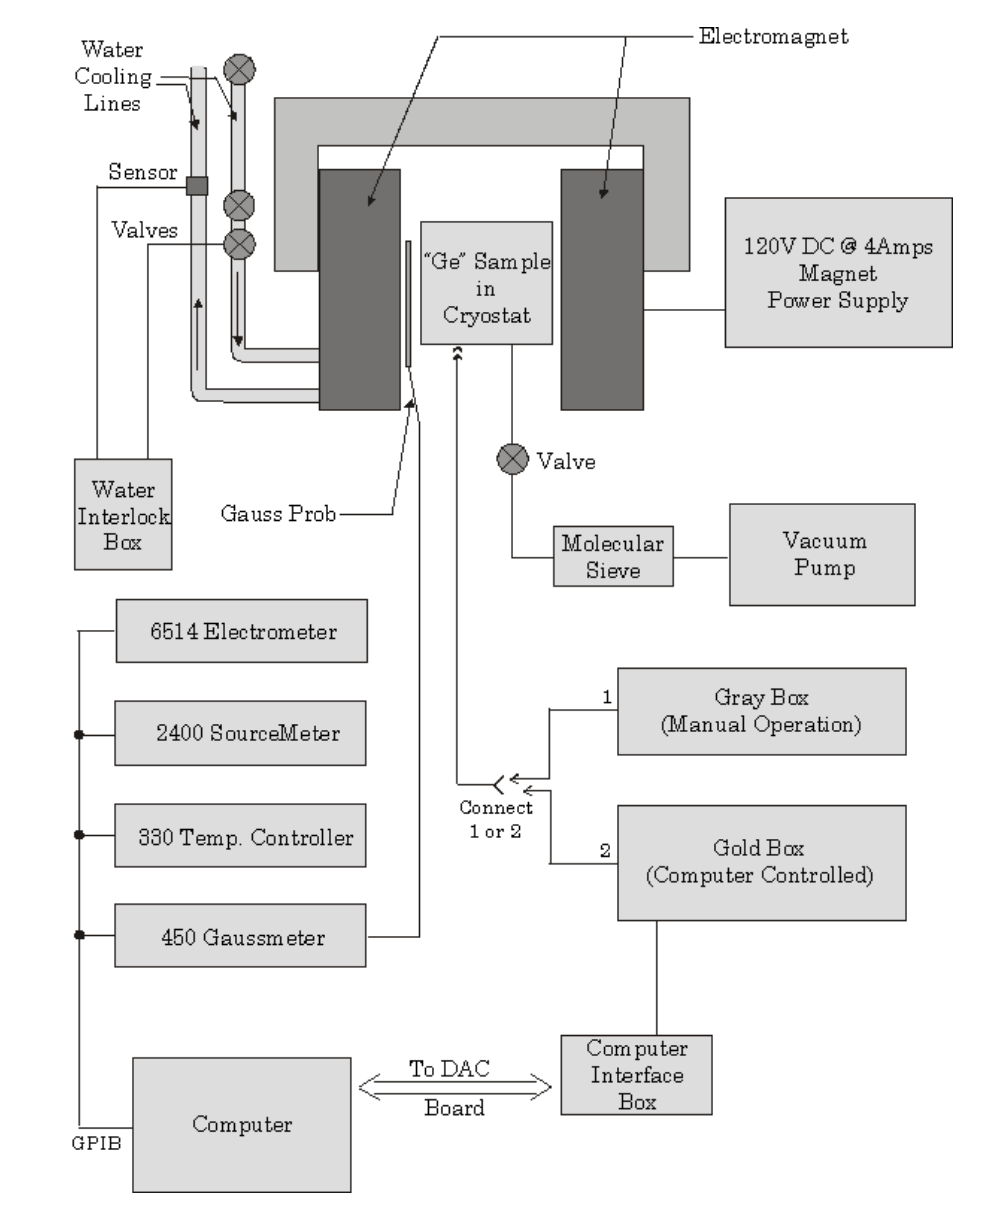
\includegraphics[scale=0.5]{images/setup-3.png}
		\caption{Macroscopic setup of the experiment apparatus. The germanium sample here is shown in the
			middle, with the vaccuum and other relevant electronic equipment surrounding it. The measurements are
			made by all the meters in the bottom left, which  are sent to the computer and compiled together in a
			\texttt{.csv} file. The reason I put this figure here is because it was too big, so it made more
		sense to include it here.}
		\label{setup-3}
	\end{figure}

	\pagebreak
	\section{Calculating Carrier Mobilities}
	\label{B}
	As mentioned in the analysis section, a large part of the logic in the analysis section is driven by the
	work of \cite{melissinos}, and in this section we will present their logic in full. To begin,
	\cite{melissinos} (and also the
	equation we derive in section \ref{multiple-carriers}) provides the
	following equation for the Hall coefficient \( R_H \) in the case where there are two carriers present:
	\[
		R_H = \frac{\mu_p^2 p - \mu_e^2 n}{e(\mu_p p + \mu_e n)^2}
	\]
	This is a more complex formula than the one we introduce in the theory section; this is because when
	there is more than one charge carrier present, the Hall effect acts differently on the positive and
	negative carriers, so as a result the equation for \( E_H \) and \( J_x \), giving us a more complicated
	equation. It is important to note that aside from a minus sign, this equation does collapse into equation
	\ref{rh} when we set either \( n \) or \( p \) to zero. 

	Now, given this relation, for \( p \) type semiconductors, we have \( p \) to be nonzero, so it now makes
	sense that \( R_H \) should equal zero at some point (as in, it's a physical point). 
	At the point where \( R_H \) equals zero, then we
	have the following relation:
	\[
		\mu_p^2 p - \mu_e^2 n = 0 \implies n\left( \frac{\mu_e}{\mu_p} \right)^2 - p = 0
	\]
	Fro here on, we now denote \( b = \mu_e / \mu_p \), so this equation reads \( nb^2 - p = 0 \). Now, we
	make the simplification that in the extrinsic regime, all the doped carriers participate in conduction and
	none of the intrinsic electrons do, so we have \( p = N_a \) and \( n = 0 \) in the extrinsic regime.
	In the intrinsic regime, because the electrons and holes come in pairs, then if \( n = N \) we have \( p
	= N_a + N \). Plugging the values in the extrinsic regime into the above equation, we get:
	\begin{equation}
		\label{n-equation}
		Nb^2 - (N_a + N) = 0 \implies N = n = \frac{N_a}{b^2 - 1} 
	\end{equation}
	This result will serve as the central equation we use to solve for \( n \) in the intrinsic regime.
	There are also other quantities that exist at \( T = T_0 \), the temperature where \( R_H = 0 \). In
	particular, from equation \ref{mobility} we can now write:
	\[
		\sigma_0 = \frac{1}{\rho} = e(n \mu_n + (N_a + n)\mu_p)
	\]
	This quantity we are directly measuring, since we compute \( \sigma = \frac{1}{\rho} \) for all \( T \). 
	We also have another equation for the conductivity, which comes from the extrinsic regime. To get the
	value at \( T = T_0 \), we extrapolate our fit in the extrinsic regime to \( T = T_0 \), which is:
	\[
		\sigma_e = \sigma(T = T_0) = e N_a \mu_p(T = T_0)
	\]
	We get the \( \mu_p \) relationship as a function of temperature by fitting it to \( T^{-n} \), which
	allows us to extrapolate \( \sigma \) to the point \( T = T_0 \).
	Now, we can take the ratios of these two at \( T = T_0 \), which gives:
	\[
		\frac{\sigma_0}{\sigma_e} = \frac{n \mu_n + (N_a + n)\mu_p}{\mu_p N_a} = 
		\frac{N_a + n(1 + b)}{N_a} = \frac{b}{b - 1}
	\]
	where the last equality comes from substituting equation \ref{n-equation} to get the ratio in terms of \(
	b\) only. From here, we may solve for \( b \):
	\[
		b = \frac{\sigma_0}{\sigma_0 - \sigma_e} = \frac{1}{1- \frac{\sigma_e}{\sigma_0}}
	\]
	Then, with \( b \) determined, we can now go back to equation \ref{n-equation} and solve for \( n \),
	which completes the analysis. Here, hopefully it is clear to see why we need the assumption that \( p =
	N_a \) in the extrinsic regime. Without this assumption, we would not be able to write a nice expression
	for \( n \) and we also wouldn't be able to write a nice expression for \( \sigma_0 / \sigma_e \) either. 

	\pagebreak

	\section{Data}
	Because the raw dataset is rather large for this lab, so instead of pasting these all into this document,
	I will instead attach a link to the dataset instead. You can find the full dataset along with the
	relevant plots using:
	\url{https://drive.google.com/drive/folders/1DcLZfVUPI55-ZmGKXyVG6E5kIr6W5yFh?usp=drive_link}


\end{document}
